\documentclass{beamer}
\usepackage[utf8]{inputenc}
\usepackage{graphicx}

\hypersetup{
    colorlinks,%
    citecolor=blue,%
    filecolor=blue,%
    linkcolor=blue,%
    urlcolor=blue 
    %urlcolor=mygreylink     % can put red here to better visualize the links
}

\author[Sowmya Vajjala]{Instructor: Sowmya Vajjala}

\title[LING 520]{LING 520: Computational Analysis of English}
\subtitle{Semester: FALL '16}

\date{22 September 2016}

\institute{Iowa State University, USA}
%%%%%%%%%%%%%%%%%%%%%%%%%%%

\begin{document}

\begin{frame}\titlepage
\end{frame}

\begin{frame}
\frametitle{Class outline}
\begin{itemize}
\item morphological analysis - comments %10min
\item Probability overview %20 min (and about how to get them in code)
\item ngrams and language models %20min (along with smoothing etc)
\item practice exercise %here, I can ask them to use one of the lm toolkits?
\end{itemize}
\end{frame}

\begin{frame}
\frametitle{Stemming and Lemmatization - Comments}
What are your observations about those different stemmers and lemmatizers in NLTK?
\begin{itemize}
\item How similar or different do those stemmers look in terms of the output you get?
\item How is the lemmatizer different from stemmers?
\end{itemize}
\end{frame}

\begin{frame}
\begin{center}
\Large Probability Overview
\end{center}
\end{frame}

\begin{frame}
\frametitle{What is probability?}
\begin{itemize}
\item Probability of an event is a mathematical way of predicting the chance that the event will occur in the given background.
\item If I toss a coin once, what is the probability that I see a head? \pause
\item Sample space (S): All possible occurrences of a event. In this coin toss example, there are two possibilities: head, tail.
\item Event: each one of those possible occurrences can be one event. Having heads is one event, having tails is one event.
\end{itemize}
\end{frame}

\begin{frame}
\frametitle{What is probability? - Some Formulae}
\begin{itemize}
\item Probability is a number between 0 to 1. \pause
\item If there are two possible events (E1,E2) in a sample space, P(E1) + P(E2) = 1. \pause
\item P(S-E1) = 1-P(E1) \pause
\item P(A$\cup$B) = P(A) + P(B) - P(A$\cap$B) \pause
\end{itemize}
\end{frame}

\begin{frame}
\frametitle{What is probability? - Examples}
\begin{itemize}
\item In our class, there are 12 or 13 people. 
\item If I have to randomly (and unbiasedly) pick one person to present on stemming now, what is the probability that it is Lena? \pause Answer: 1/13
\item What is the probability that it will be Lena or Kim? \pause Answer: 1/13 + 1/13 = 2/13 (it is a either or case). P(A$\cap$B) is zero here. 
\item What is the probability that I pick either a second year ALT student or an American student? \pause
\\ Formula: P(2nd year ALT student) + P(American student) - P(2nd year ALT students who are americans).
\end{itemize}
\end{frame}

\begin{frame}
\frametitle{What is probability? - Examples}
\begin{itemize}
\item Look at this age distribution for 10 students: 
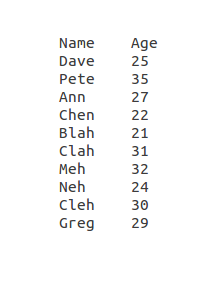
\includegraphics[width=0.3\textwidth]{prob1.png}
\item If I randomly pick one person, what is the probability that this person is below 30 years of age? \pause Ans: 6/10
\item If I randomly pick one person, what is the probability that it is Dave? what is the probability that this is not Dave? \pause Ans: 1/10 and 9/10.
\end{itemize}
\end{frame}

\begin{frame}
\frametitle{Conditional probability}
\begin{itemize}
\item Conditional probability is the probability of one event happening, when we know some other event has happened before.
\item If one of my events is seeing 2 when I roll a die (E1), the other event is seeing an even number (E2), then, P(E1$|$E2) is: 1/3. Why?? \pause
\item What is P(E1)? \pause 1/6
\item What is P(E2)? \pause 3/6 i.e., 1/2
\item What is P(E1, given E2) \pause E2 has three possibilities (2,4,6). So, probability of getting 2 is 1/3.
\end{itemize}
\end{frame}

\begin{frame}
\frametitle{Joint probability}
\begin{itemize}
\item Probability that two events occur together. Represented as P(A,B) and is the same as P(B,A)
\item So what is the difference between joint and conditional probability? \pause
\item Useful example: \url{https://goo.gl/9MVM78} \pause
\item Summary: Conditional probability is not commutative P(A$|$B) != P(B$|$A)
\item P(A,B) = P(A$|$B)*P(B) =  P(B$|$A)*P(A)
\end{itemize}
\end{frame}

\begin{frame}
\frametitle{Bayes Theorem}
\begin{itemize}
\item P(A $|$ B) = P(B $|$ A)* P(A) / P(B)
\item Example: P(Tag$|$Word) = P(Word$|$Tag)*P(Tag)/P(Word)
\item P(Word) and P(Tag) are probabilities of seeing the Word or Tag in your language corpus, independent of each other.
\item What are P(Tag$|$Word) and P(Word$|$Tag)? \pause
\item P(Tag$|$Word) is the posterior probability. P(Word$|$Tag) is called the likelihood. P(Tag) is prior. P(Word) is evidence.
\end{itemize}
Ref: An explanation of this terminology: \url{https://goo.gl/bFwcHG}
\end{frame}

\begin{frame}
\frametitle{Probability: Summary}
\begin{itemize}
\item Probability is a number between 0 and 1.
\item Joint probabilities are different from Conditional probabilities.
\item P(A$|$B) != P(B$|$A)
\item Bayes theorem: P(A $|$ B) = P(B $|$ A)* P(A) / P(B)
\end{itemize}
Note: I am only telling you what I want you to know to understand the rest of this class.
\end{frame}
%Useful links:
%http://www.mathgoodies.com/lessons/vol6/conditional.html
%https://www.cs.utah.edu/~fletcher/cs6957/lectures/ProbabilityCrashCourse.pdf
%http://cbmm.mit.edu/sites/default/files/documents/probability_handout.pdf
%http://cs.au.dk/~mailund/slides/ML07/probability-and-stats-intro.pdf
%introduce: Sample space, Events, Probability
%introduce:

\begin{frame}
\begin{center}
\Large ngrams and language models
\end{center}
\end{frame}

\begin{frame}
\frametitle{What are ngrams?}
\begin{itemize}
\item Ngram is a token sequence of N words/tokens.
\item Bigrams are two token sequences, trigrams are 3 token sequences etc.
\item Ngram model: is a probabilistic model of language, that predicts the next word based on the previous words. 
\item Order is important. So, a sequence like "I am liking this class because ..." will get more probability in a language model for English than "this liking class I am because..."
\end{itemize}
\end{frame}

\begin{frame}
\frametitle{Where are ngrams and ngram models useful?}
\begin{enumerate}
\item In any task where we need to identify words in the presence of noisy input.
\item In speech recognition, to identify which of the similar sounding words is the word being spoken in the given context.
\item In handwriting recognition and optical character recognition, to disambiguate words or characters that are not clearly identified.
\item Machine translation: choosing from a possible set of word orderings between source and target translation.
\item Spelling and grammar correction: doing context sensitive spelling and grammar check.
\item POS tagging, natural language generation, predictive text input.. and many more.
\item Non modeling use: Doing corpus analysis.
\end{enumerate}
\end{frame}

\begin{frame}
\frametitle{Where may they fail?}
\begin{itemize}
\item When there is a relatively free word-order language
\item When there is a lot of word inflection
\item When we need some deeper linguistic analysis (at the level of syntax, discourse etc)
\item When there are tons of possible spelling variations possible.
\item When you create your language model for one language, but use it for another language, or with totally new vocabulary etc.
\end{itemize}
\end{frame}

\begin{frame}
\frametitle{Constructing ngram models}
\begin{itemize}
\item Start with counting ngram sequences in a large corpora.
\item goal: predict the next word based on some context. E.g., what is most likely to occur after "Ngram is a sequence of "
\item In terms of probabilities:
\begin{enumerate}
\item If "ngram is a sequence of" is the context or history
\item Let us say there is an english word "whatever"
\item ngram model should estimate P("whatever"$|$"ngram is a sequence of")
\item How can we get this probability? 
\end{enumerate}
\end{itemize}
\end{frame}

\begin{frame}
\frametitle{Probability of Language}
\begin{itemize}
\item If we have a representative corpus of the style of language you want to see, 
\item If you have a program to count the frequency of occurrence ngrams of varying sizes,
\item then, P(whatever$|$ngram is a sequence of)  = C(ngram is a sequence of whatever$|$ ngram is a sequence of)
\end{itemize}
Sounds pretty straight forward, doesn't it?
\end{frame}

\begin{frame}
\frametitle{Probability of Language}
\begin{itemize}
\item With this approach, if you have a large enough corpus, you can reliably estimate the probability of any sequence of words in a language.
\item But, there are a few issues:
\begin{enumerate}
\item Language is creative. New forms of word combinations keep coming up. No corpus can cover everything. \pause
\item Most of the sentences will have a zero probability, if there is one new word in it, or one unusual usage. \pause
\item Imagine writing a program for counting 2--10 ngrams and storing all this info, for such a large corpus! \pause
\item .. and then imagine how to quickly retrieve this count information from those millions of ngrams you will have!
\end{enumerate}
\end{itemize}
\end{frame}

\begin{frame}
\frametitle{The chain rule of probability}
\begin{itemize}
\item Here is one way of combining joint and conditional probabilities to estimate a sentence probability.
\item If we assume a sentence S to be a sequence of words (w1, w2, .... wn), then, the probability of this sentence will be:
\item P(S) = p(w1$|$beginning of sentence)*p(w2$|$w1)*p(w3$|$w1,w2)*p(w4$|$w1,w2,w3)*... ... ... *p(wn$|$w1,w2,w3...wn-1)
\item This is perhaps a better representation, but is not making our job of counting ngrams any easier!
\item One solution: markov assumption
\end{itemize}
\end{frame}

\begin{frame}
\frametitle{The Markov assumption}
\begin{itemize}
\item What is it?: It says instead of computing probabilities using entire history, we can use only the last few previous words.
\item P(whatever$|$ngram is a sequence of) can be approximated as P(whatever$|$sequence of) if we choose a trigram model (2 words before current word).
\item P(whatever) - unigram model. P(whatever$|$of) -bigram model .. and so on. 
\end{itemize}
\end{frame}

\begin{frame}
\frametitle{A Bigram Language Model}
\begin{itemize}
\item This is the formula for getting bigram probabilities for one word: P(w$_n|$w$_{n-1}$) = C(w$_{n-1}$,w$_{n}$)/$\Sigma_w$(w$_{n-1}$w) \pause
\item However, $\Sigma_w$(w$_{n-1}$w) just means C(w$_{n-1}$). Why? \pause
\item The problem of several bigram combos being zero is still not resolved. Since our formula has a multiplication, this can potentially give zero probability to any given sentence even if there is only one bigram with zero probability. We will discuss how to address that part on tuesday.
\end{itemize}
\end{frame}

\begin{frame}
\frametitle{An Example}
\framesubtitle{Source: Section 4.2, Page 89 in J\&M}
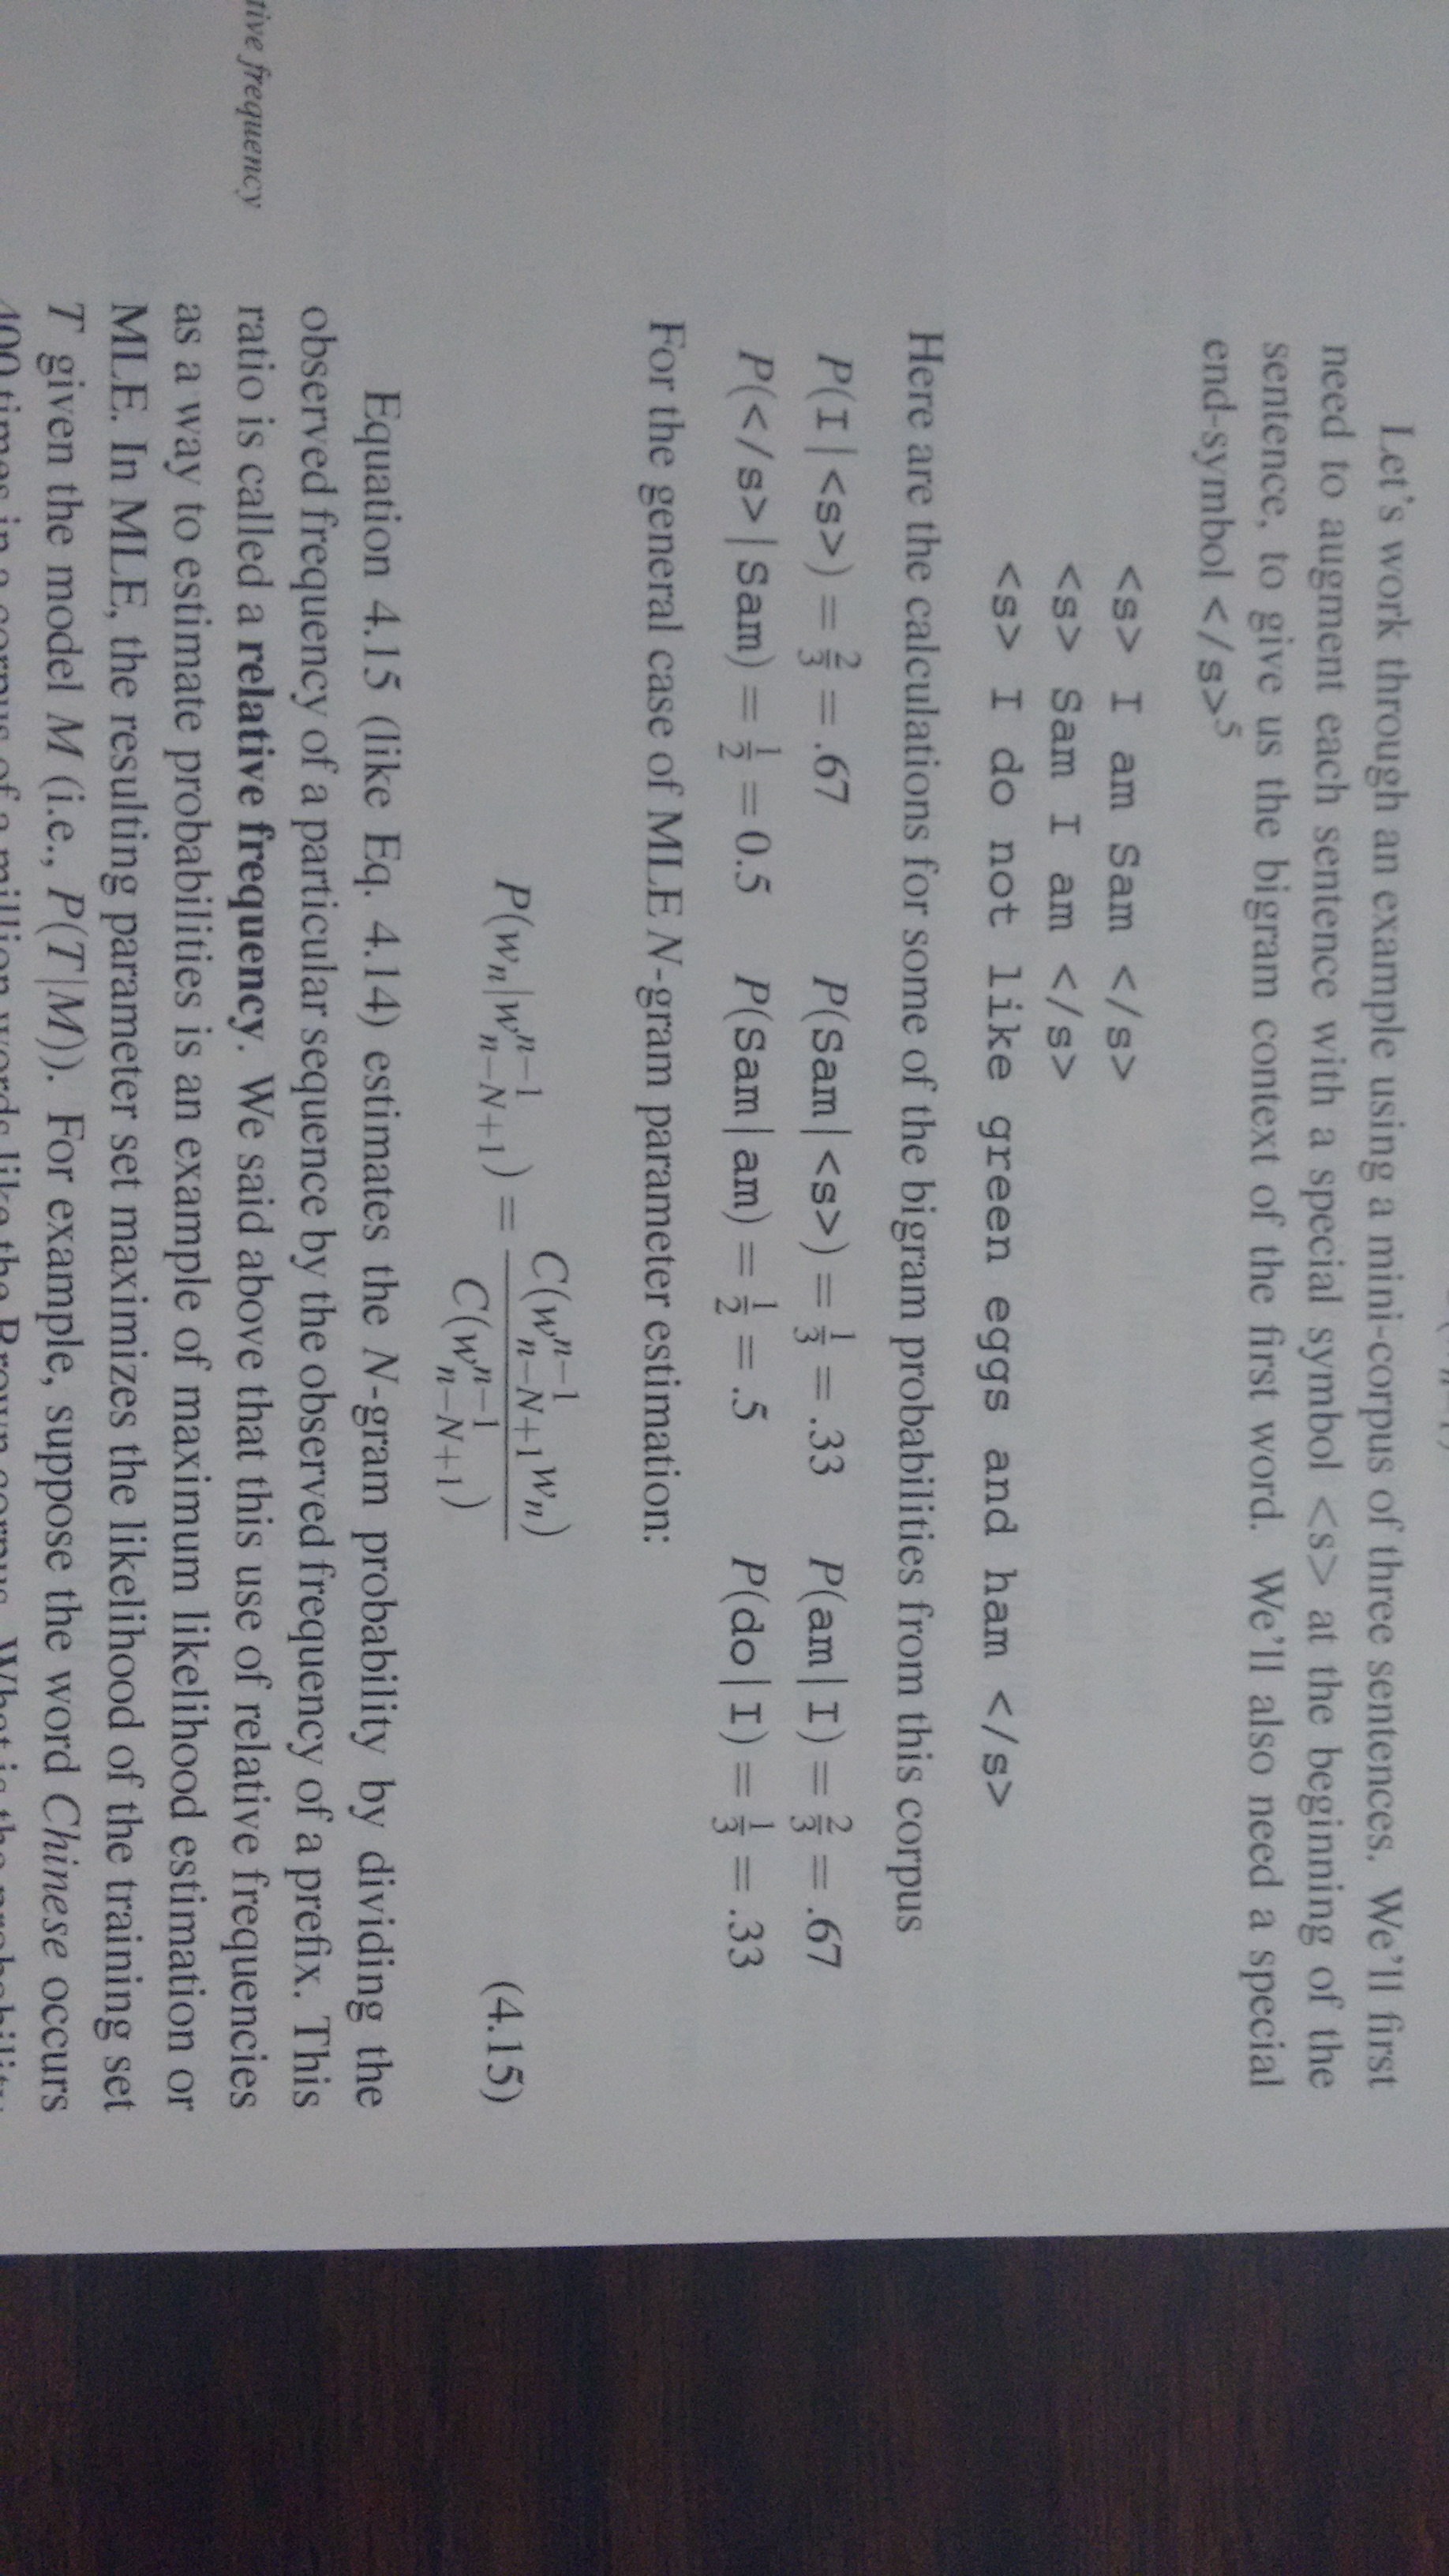
\includegraphics[width=0.7\textwidth,angle=90]{ngramprobs.jpg}
\end{frame}

\begin{frame}
\frametitle{Practice Exercise}
Go to the following url, follow the python code snippets given there, and understand what is happening at each step. You can work in groups of 3. \url{https://goo.gl/U1ghTw}. I would expect one or two groups to give a summary of what they understood, in Tuesday's class.
\end{frame}

\begin{frame}
\frametitle{Next Class}
\begin{itemize}
\item Topics: continuation of language models
\item ToDo:
\begin{enumerate}
\item Read this article on Language Modeling in Python by Nitin Madnani (\url{http://desilinguist.org/pdf/langmodel.pdf}). We will start the next class with a discussion on this. Please do read.
\item Watch Week 6 Lectures by Radev.
\end{enumerate}
\end{itemize}
\end{frame}
\end{document}


\begin{frame}
\frametitle{Problems with this model}

\end{frame}

\begin{frame}
\frametitle{Smoothing}
%4.2-4.6 - 30 min
\end{frame}

